\section{Introduccion}


Se lleva a cabo la implementación de los siguientes 5 filtros:

\begin{center}
 \begin{tabular}{cccc}
   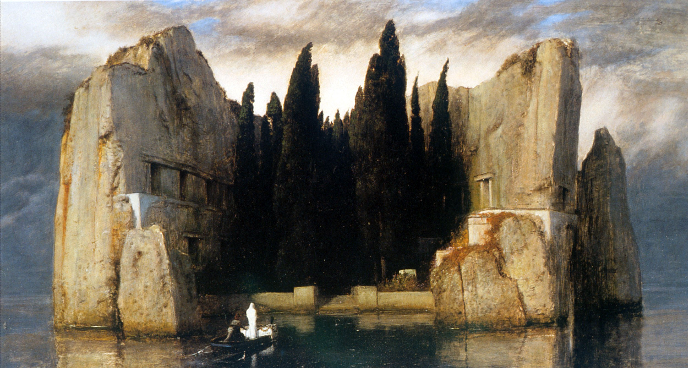
\includegraphics[width=0.2\textwidth]{imagenes/island.png} &
   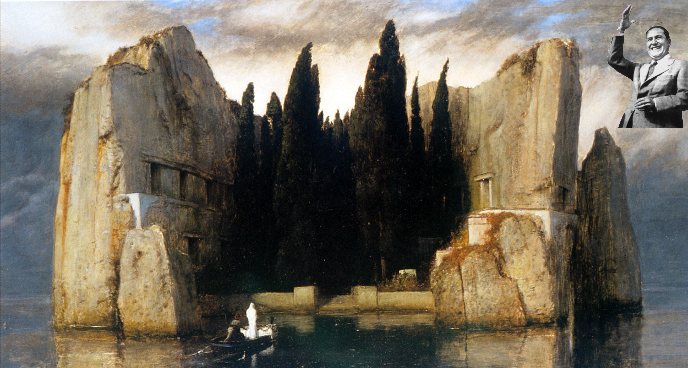
\includegraphics[width=0.2\textwidth]{imagenes/island-blit.png} &
   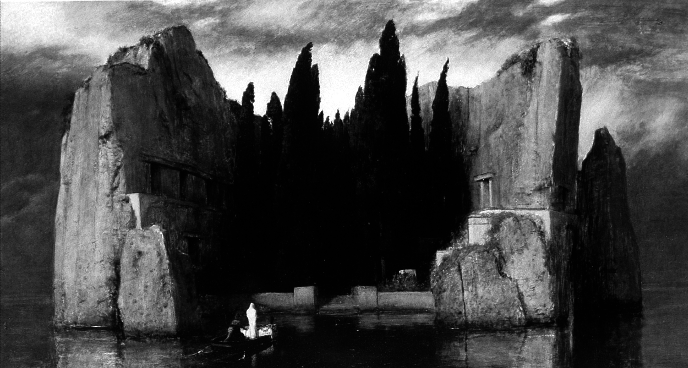
\includegraphics[width=0.2\textwidth]{imagenes/island-monocromatizar.png} \\
   Imagen original & Blit & Monocromatizar \\
   \\
   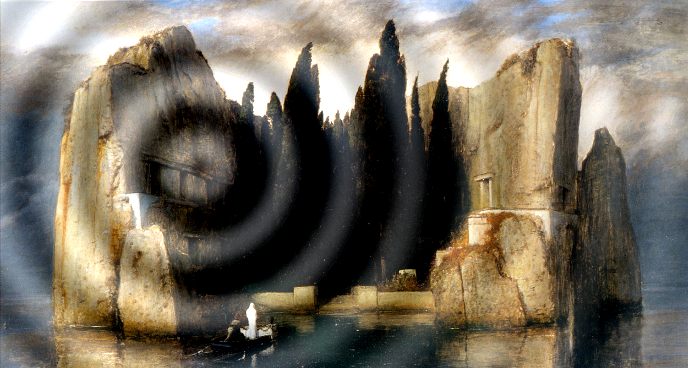
\includegraphics[width=0.2\textwidth]{imagenes/island-ondas.png} &
   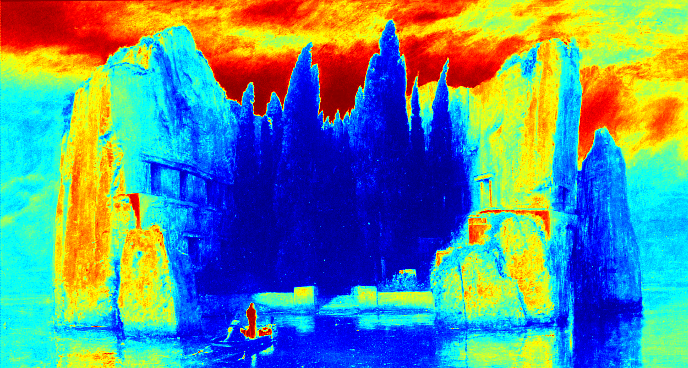
\includegraphics[width=0.2\textwidth]{imagenes/island-temperature.png} &
   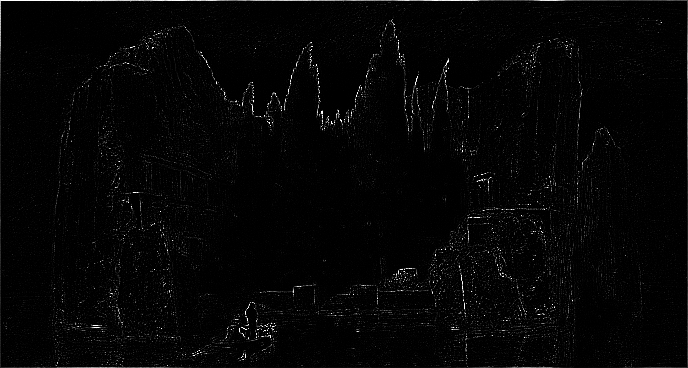
\includegraphics[width=0.2\textwidth]{imagenes/island-edge.png} \\
   Ondas & Temperature & Edge \\
 \end{tabular}
\end{center}
  
  La elaboración del trabajo se dividió en dos etapas. En primer lugar, se implementaron ambos filtros tanto en lenguaje C como en lenguaje ensamblador para la arquitectura x86-64 de Intel. En este último caso, se utilizaron las instrucciones SSE de dicha arquitectura, que aprovechan el ya mencionado modelo SIMD para procesar datos en forma paralela.

  Una vez realizadas estas implementaciones, fueron sometidas a un proceso de comparación para extraer conclusiones acerca de su rendimiento. Con este fin, se experimentó con variaciones tanto en los datos de entrada como en detalles implementativos de los mismos algoritmos. De esta manera, se pudo recopilar datos sobre el comportamiento de cada implementación, y contrastar estos resultados con diversas hipótesis previamente elaboradas.
